\documentclass[a4paper,fontsize=9.0pt]{scrartcl}
\usepackage{float}
% \usepackage[10pt]{extsizes}
\usepackage[utf8]{inputenc}
\usepackage[margin=0.9in]{geometry}
\usepackage{titling}
\usepackage{graphicx}
\graphicspath{ {./graphs/} }
\setlength{\droptitle}{-5em}

\title{\textbf{Baselines - Combating Partisan Homogenization in News Recommendation Systems}}
\date{\vspace{-10ex}}
\begin{document}
\maketitle

\tableofcontents

\newpage
\section{General Experiment Settings}
\textbf{github-url} : https://github.com/karthikshivaram24/Combatting-partisan-homogenization
\begin{flushleft}
\begin{itemize}
  \item News Articles Used : \textbf{127344}
  \item Features: \textbf{TF-IDF}
  \item Dimensionality Reduction : \textbf{SVD}
  \item Clustering Algorithm : \textbf{K-Means}
  \item Number of Clusters : \textbf{1000}
  \item Cluster Pair Filtering 
  \begin{itemize}
      \item Minimum Cluster Size : \textbf{500}
      \item Minimum Partisan Size : \textbf{0.5}(used balanced sampling to make label distributions equal)
  \end{itemize}
  \item Recommendation Model
  \begin{itemize}
      \item Logistic Regression
      \item SGDClassifier with log loss
  \end{itemize}
  \item Performance Metrics
  \begin{itemize}
      \item \textbf{Macro} : F1, precision , recall
      \item \textbf{@K} : F1, precision, recall
  \end{itemize}
  \item User Preferences:
  \begin{itemize}
      \item \textbf{Homogeneous} : Likes articles of the same partisan score across cluster pair ( Likes conservative articles in both clusters)
      \item \textbf{Heterogeneous} : Likes articles of different partisan score across cluster pair (Likes conservative articles in cluster 1 and liberal articles in cluster 2)
  \end{itemize}
\end{itemize}
\begin{figure}[H]
 \centering
 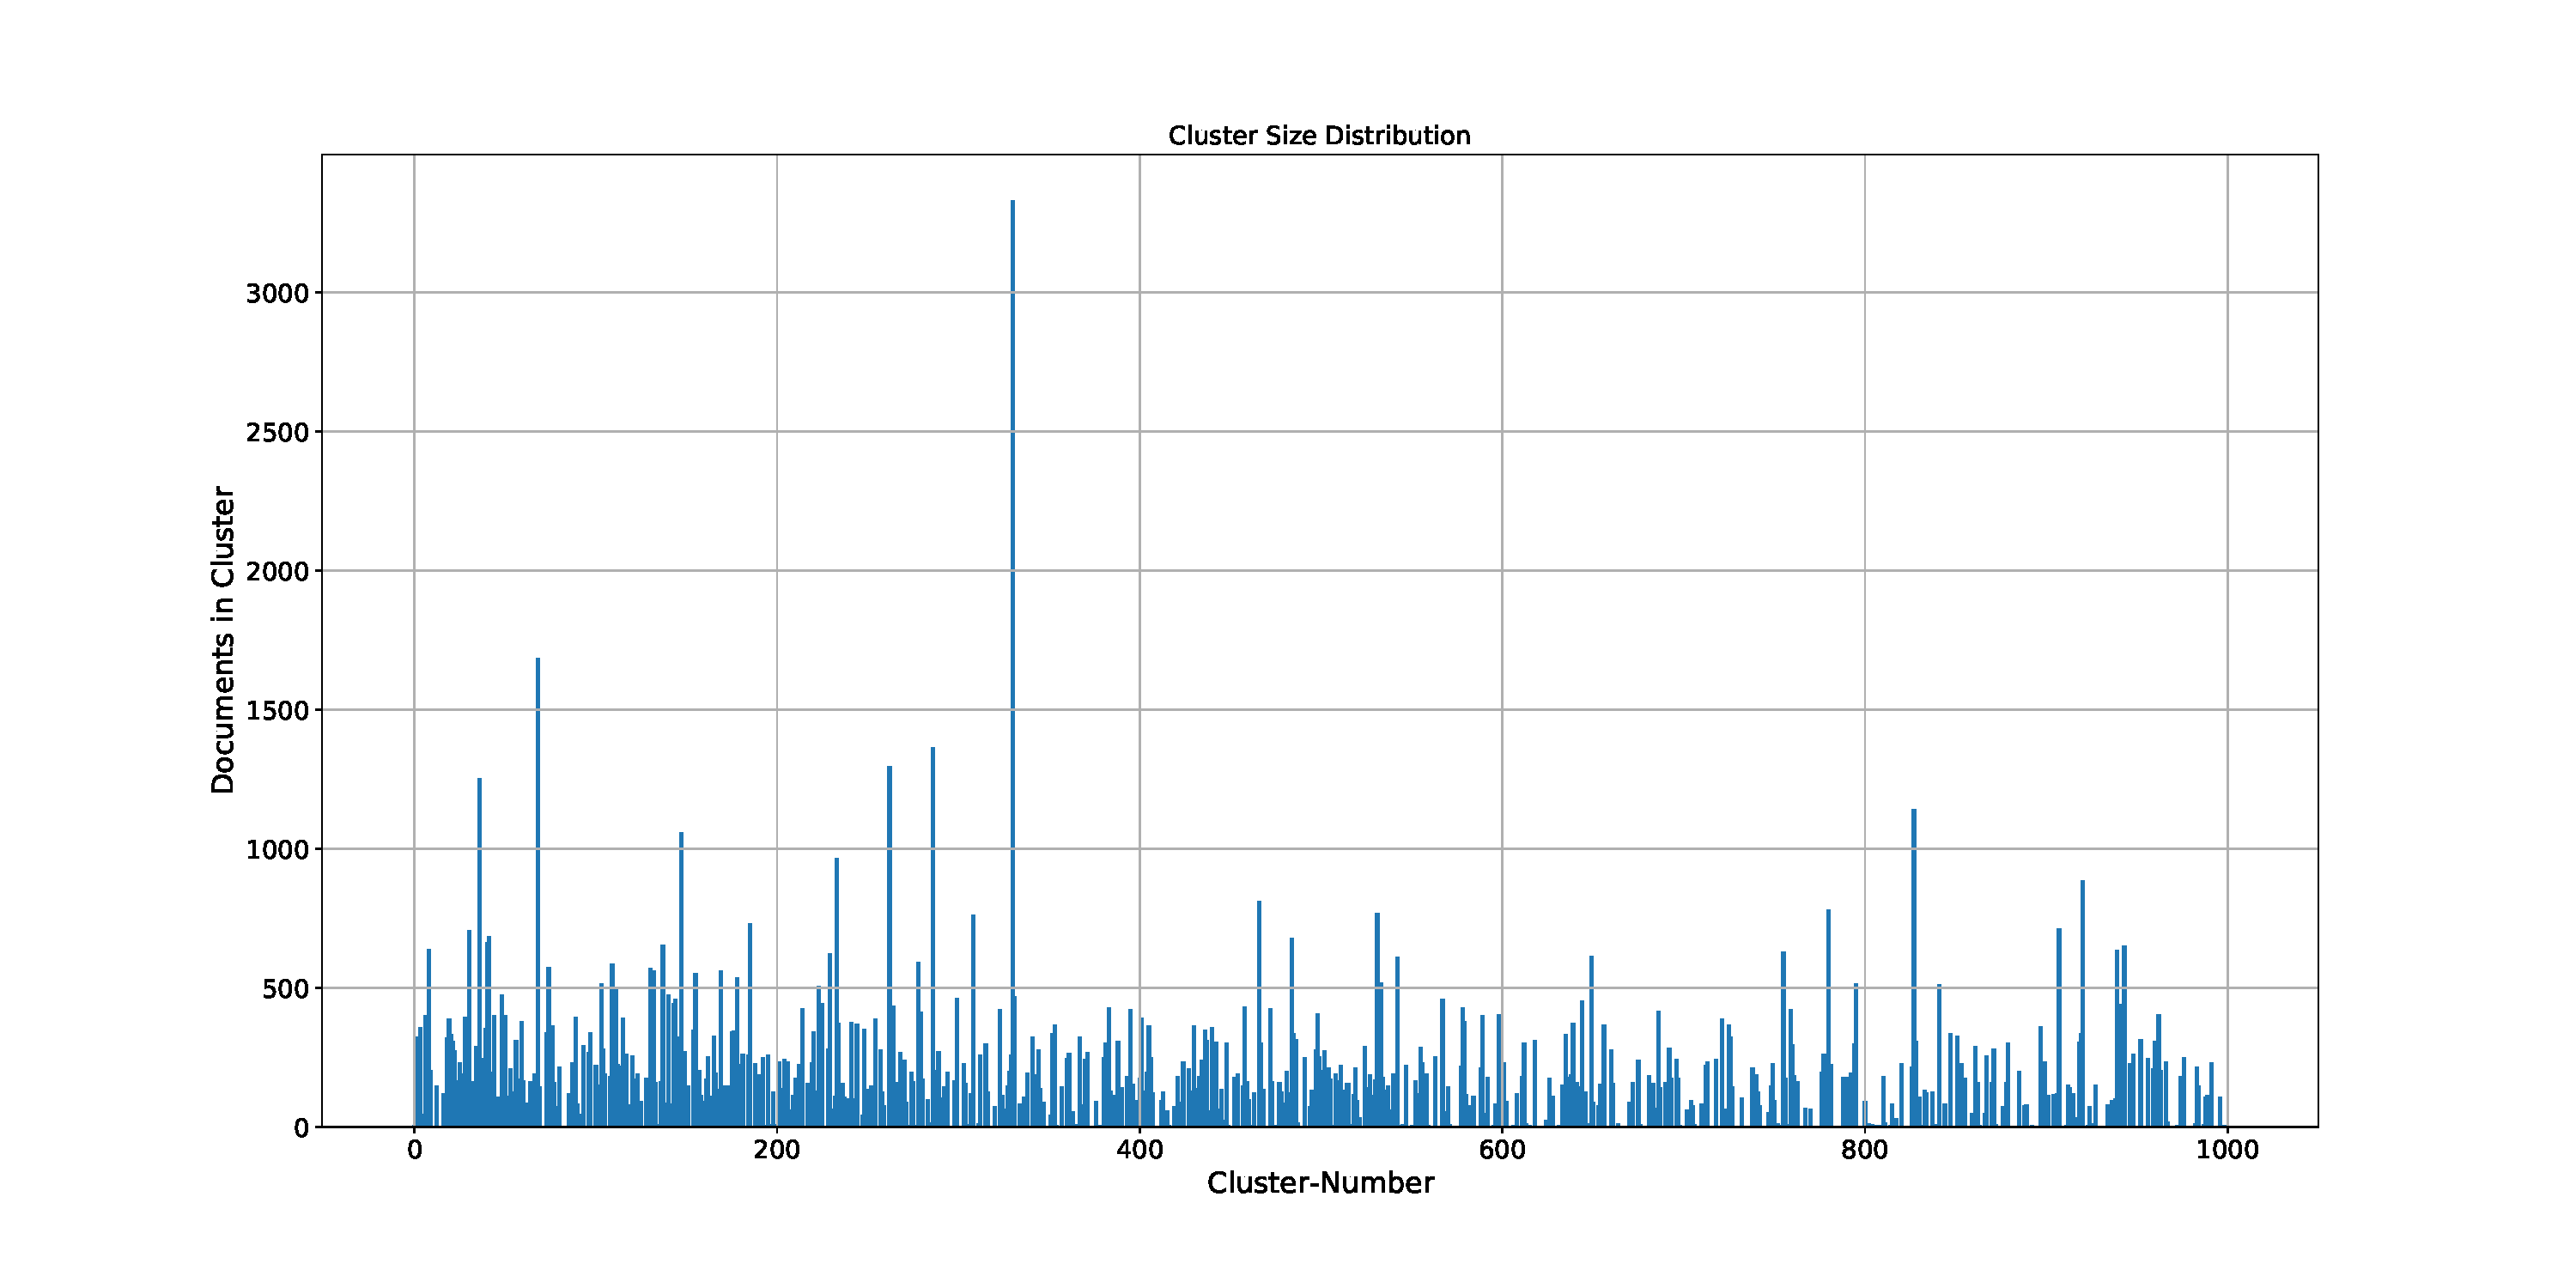
\includegraphics[width=1.0\textwidth]{Graphs/cluster_size_dist.pdf}
\end{figure}
\end{flushleft}


\newpage
\section{Baseline 1: How Topic Similarity affects Model Performance}
\begin{flushleft}
Here we want to measure how well a recommendation system performs on an unseen topic for users with different types of preferences and how this performance varies as similarity between topics increases (seen and unseen topic similarity).
\end{flushleft}
\vspace{-5ex}
\begin{figure}[H]
%  \centering
 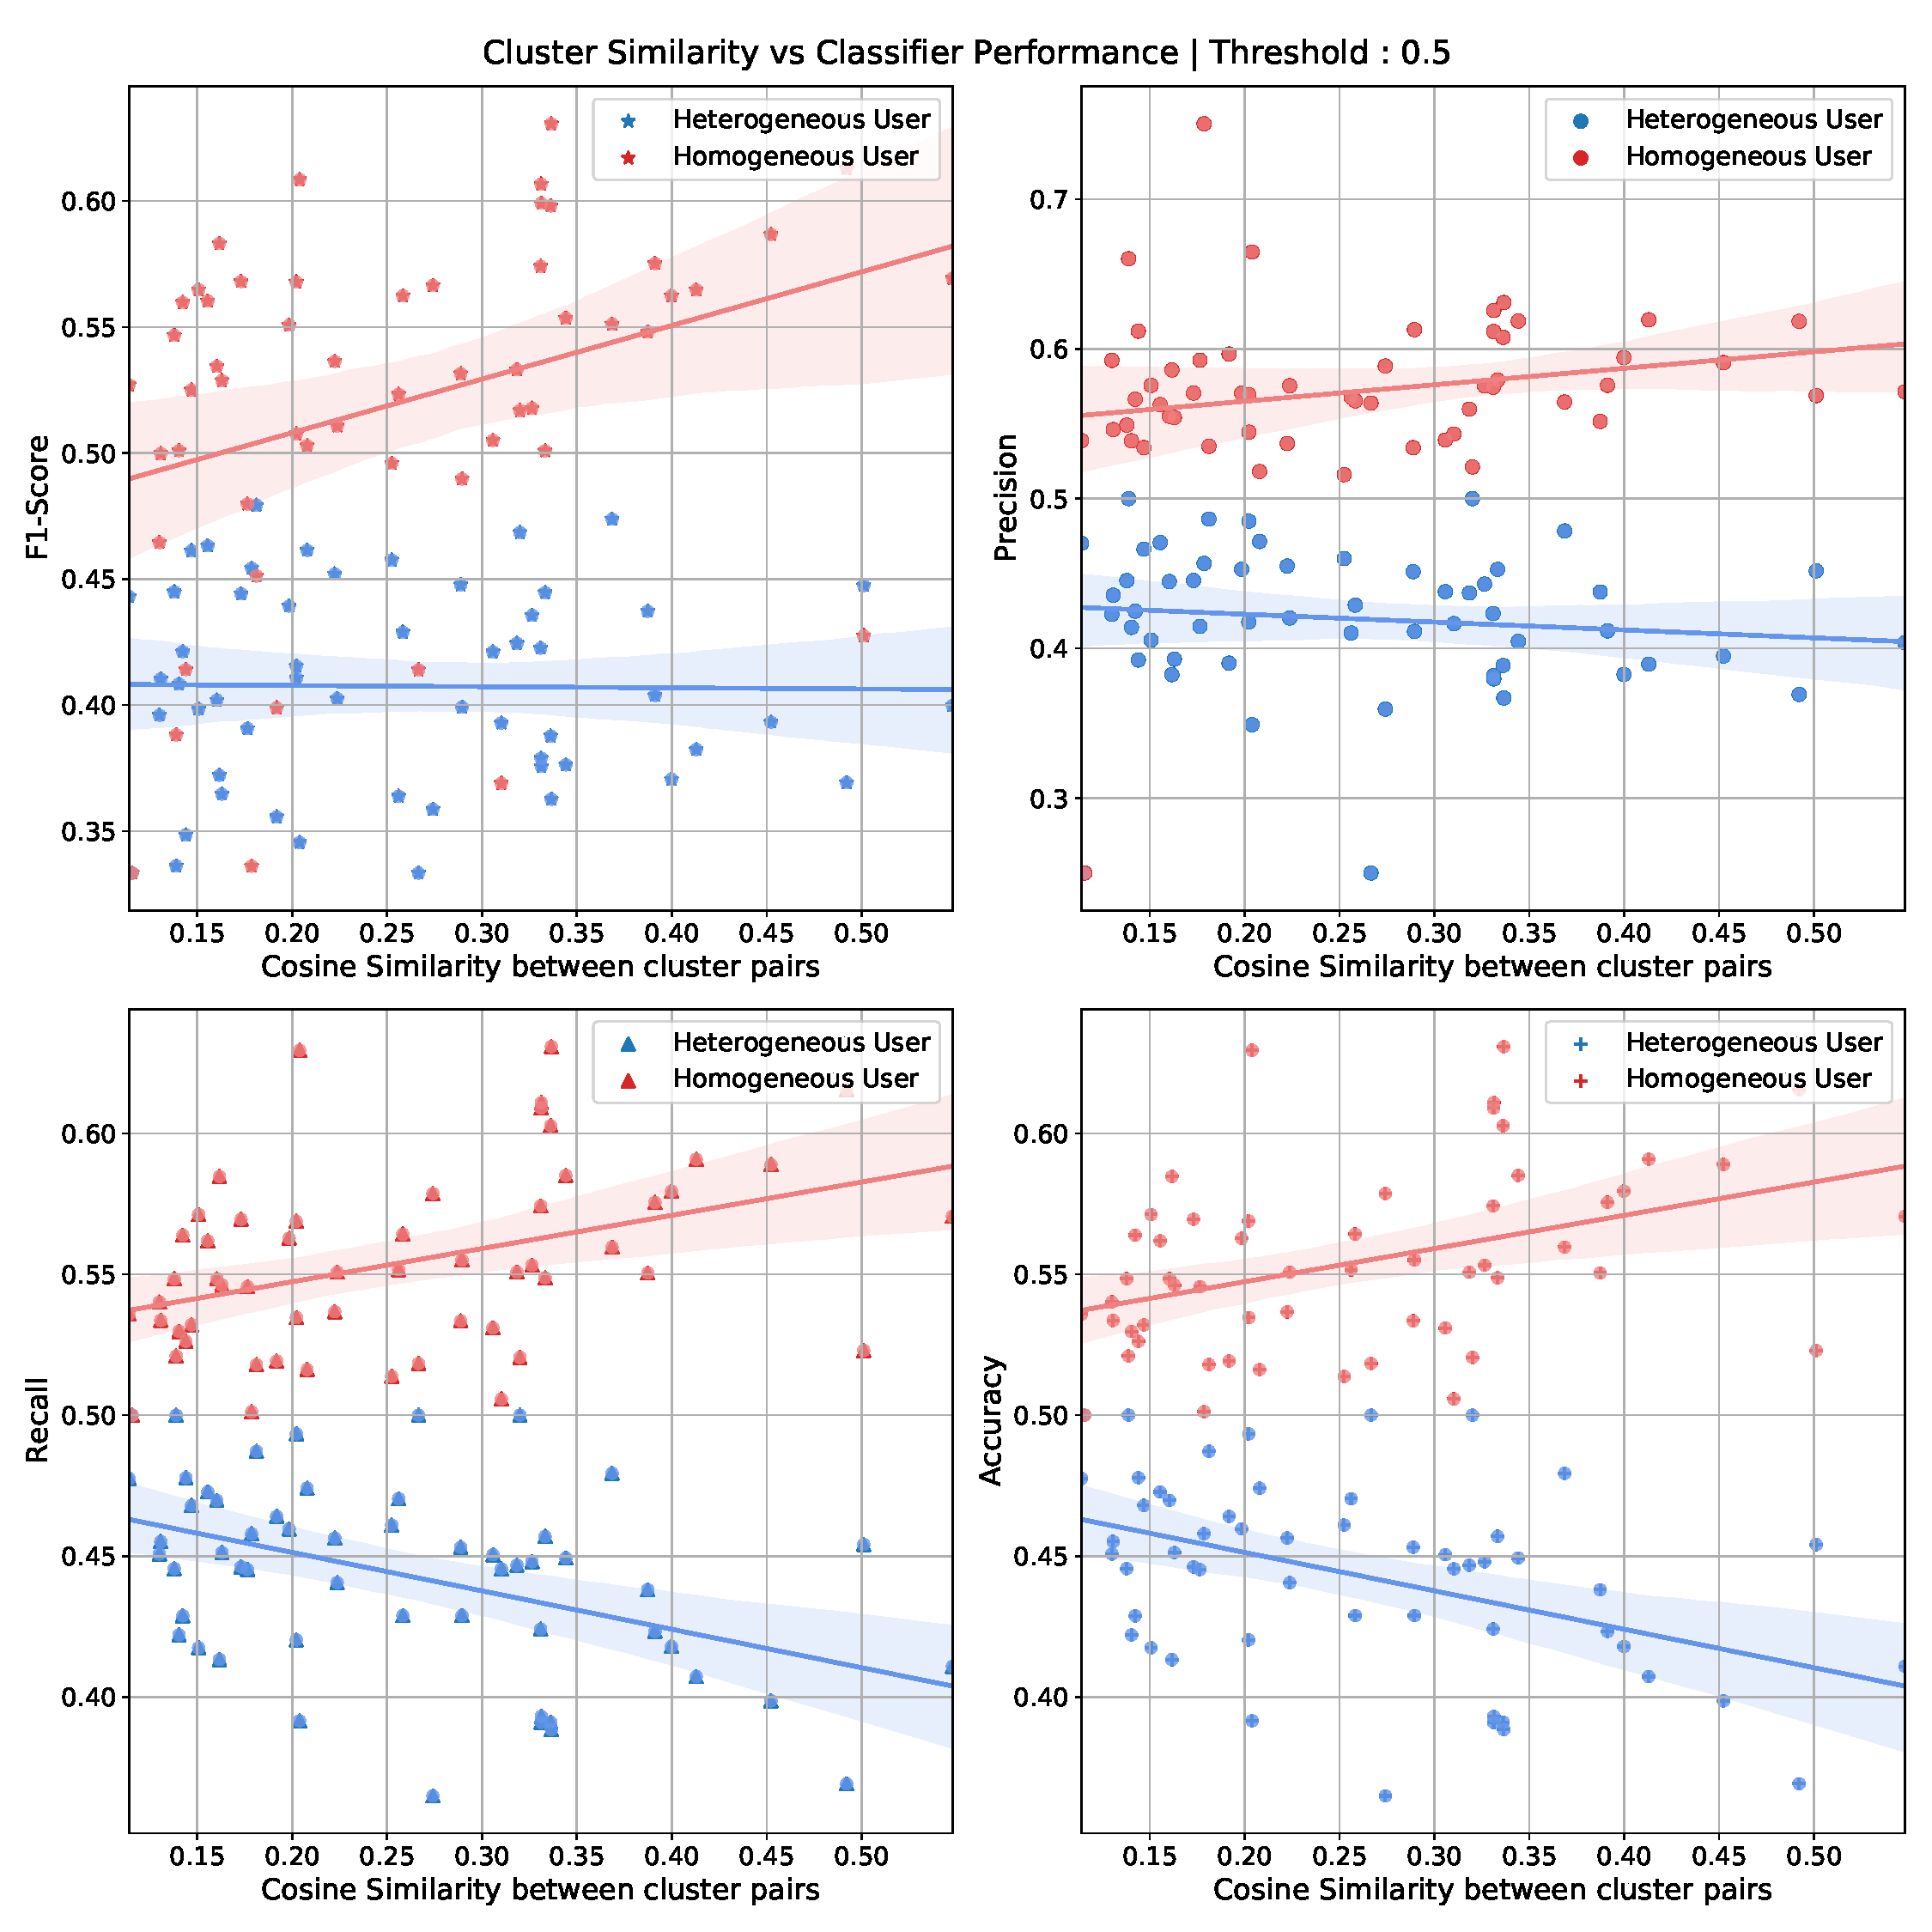
\includegraphics[width=0.6\textwidth]{Graphs/cluster_sim_vs_model_perf_5.pdf}
\end{figure}
\begin{flushleft}
We see that for Homogeneous users all the metrics increase as the similarity between topics increases, but in the case of Heterogeneous users the opposite effect takes place since the recommendation model has a harder time distinguishing between articles with different partisan scores as the similarity between topics increases.
\end{flushleft}



\vspace{-1ex}
\section{Baseline 2: Online Learning Setting}
\begin{flushleft}
To emulate a real-world scenario , we want to simulate a recommendation system interacting with a user over a set of unseen articles , slowly updating itself to the user's preferences, \textbf{N=200} is used here to calculate the metrics.
\end{flushleft}
\vspace{-3ex}
\begin{figure}[H]
 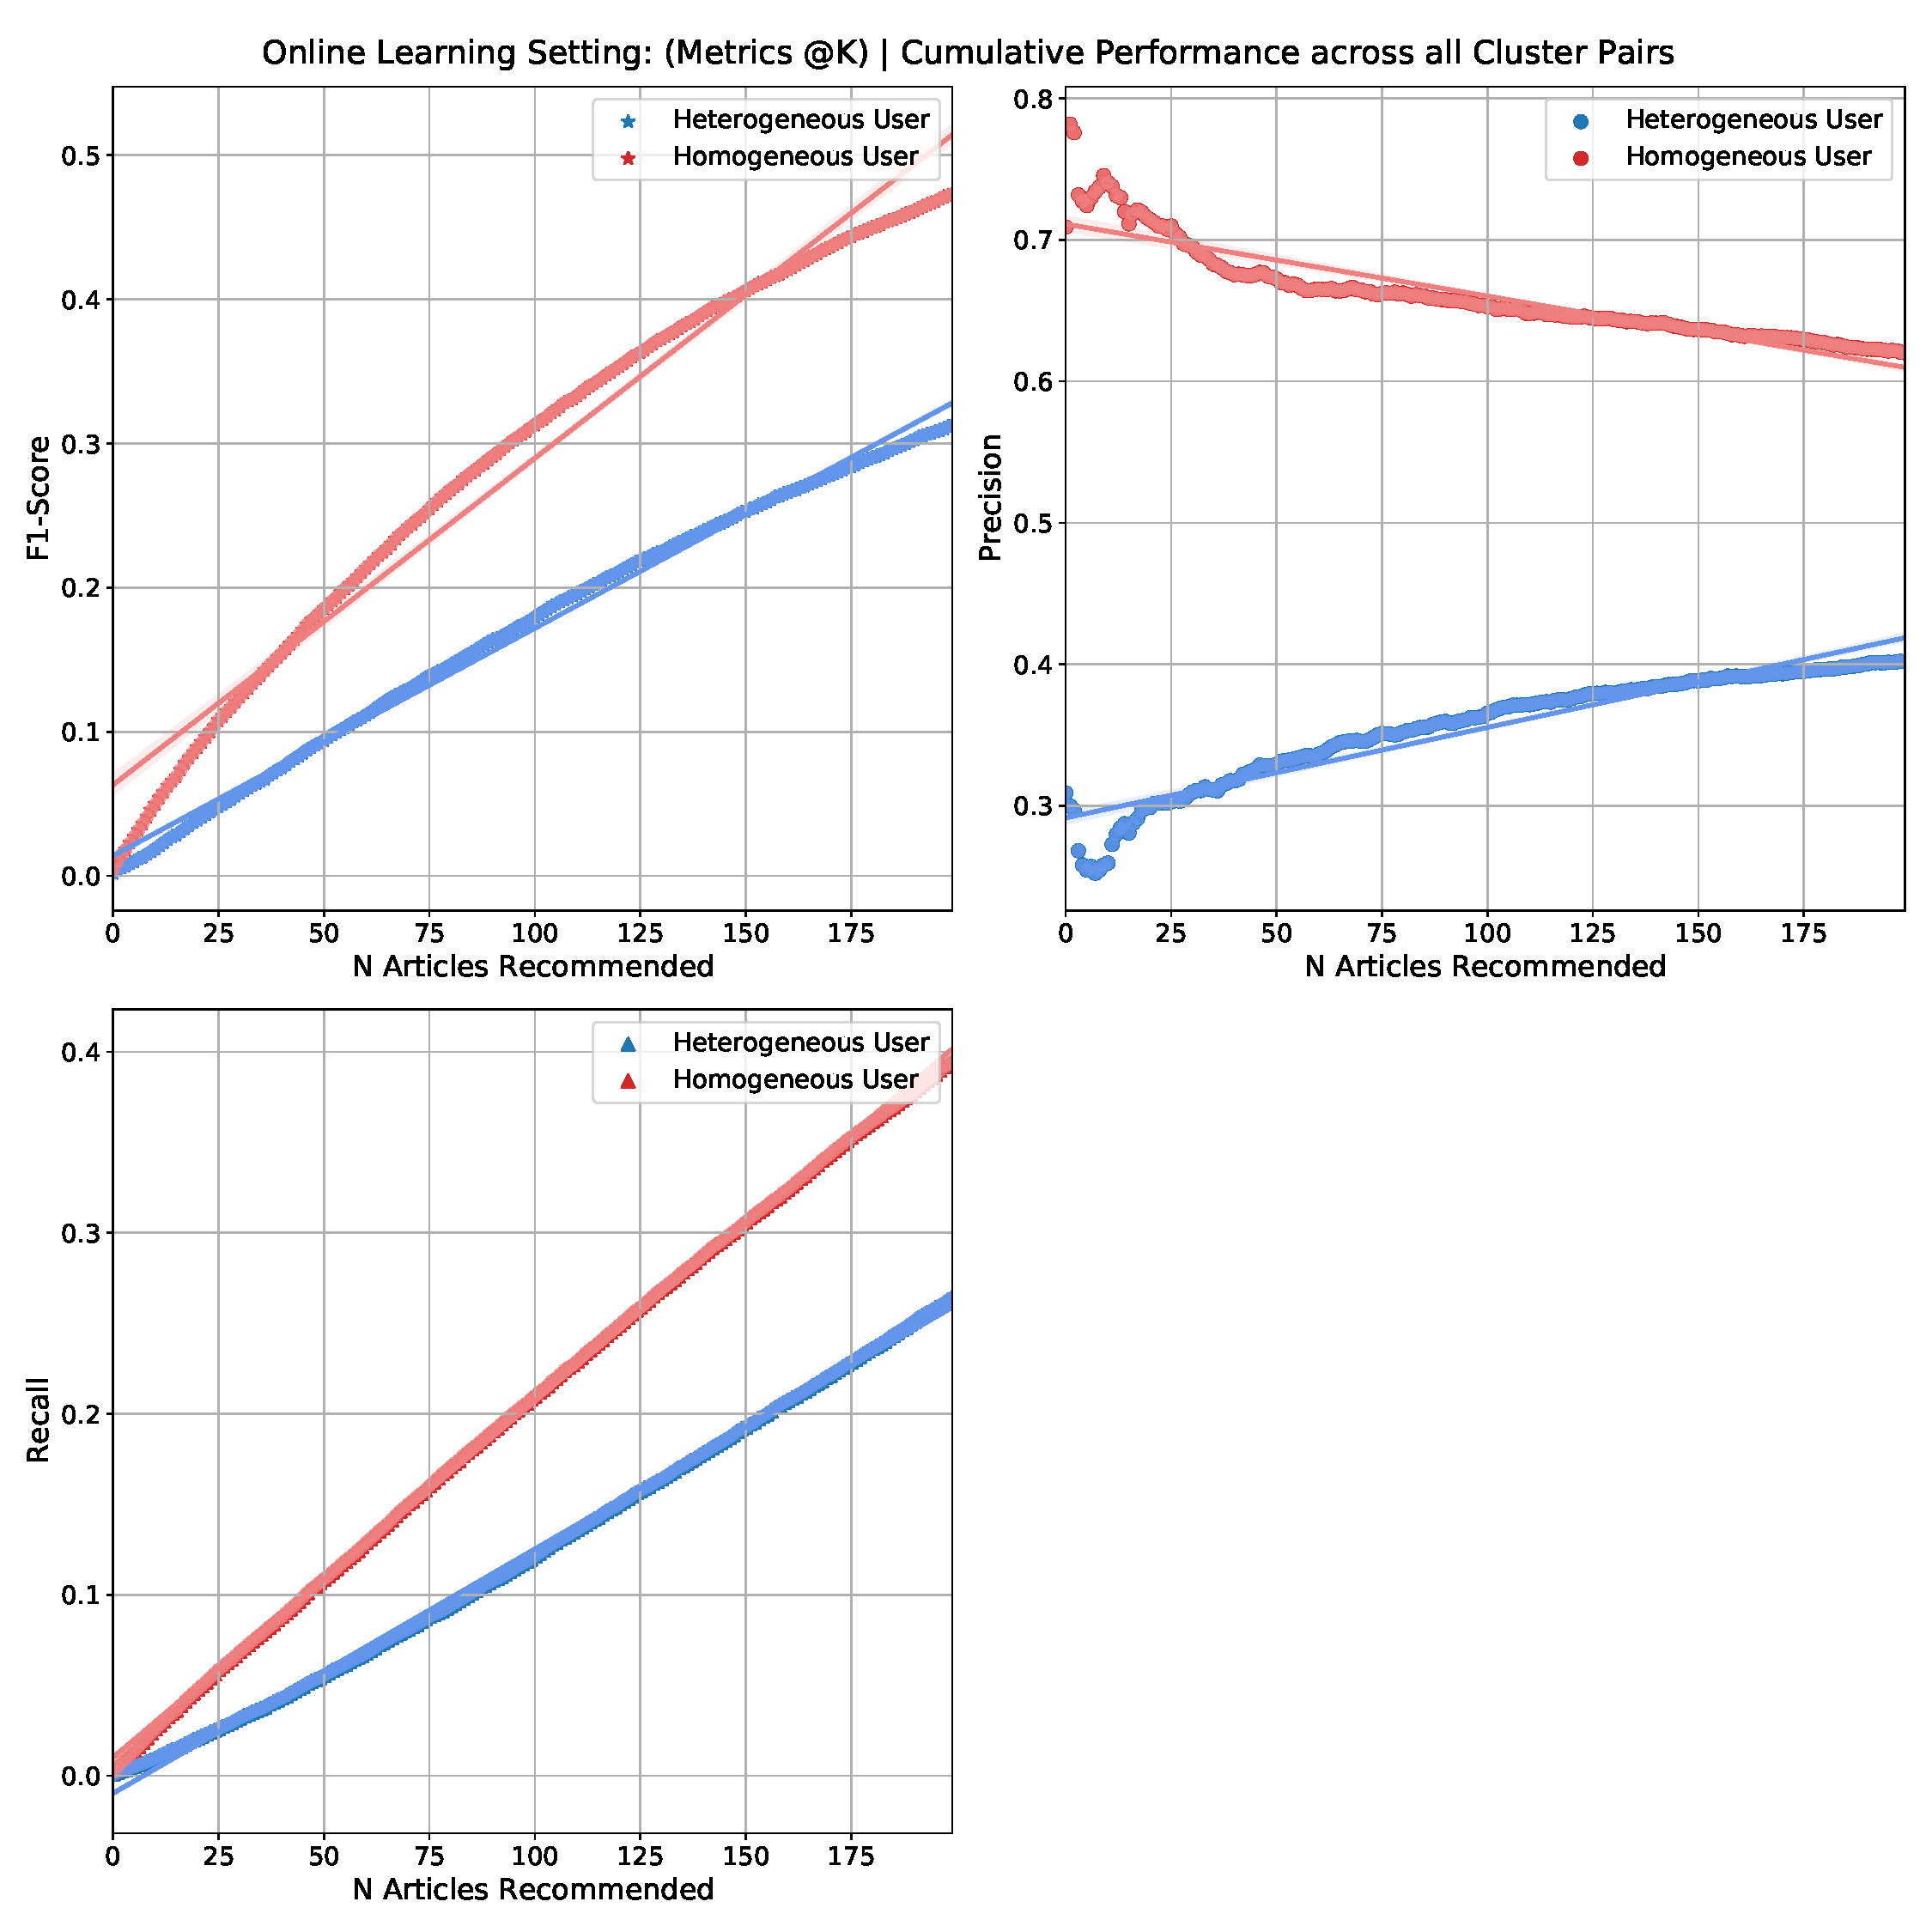
\includegraphics[width=0.6\textwidth]{Graphs/user_interaction_vs_model_performance_cumu.pdf}
\end{figure}
\begin{flushleft}
The above figure shows the mean results across all cluster pairs, here we see that the \textbf{F1@K} metric tends to increase as the recommendation system increases it's interaction with both type of users, but is lower for Heterogeneous users compared to Homogeneous users.
\end{flushleft}
\begin{flushleft}
For the \textbf{Precision@K} metric we see that there is a dip in precision for Homogeneous Users while an increase occurs for Heterogeneous Users (but there is an initial dip). The opposite occurs for \textbf{Recall@K} (Precision - Recall Tradeoff) i think varying  the classifier threshold can help us optimize one metric over the other.
\end{flushleft}


\vspace{-1ex}
\section{Baseline 3: How easy is it for the Recommendation System to detect a change in topics}
\begin{flushleft}
We want to know how the recommendation system performs in detecting a change in topics , so we measure the performance of the system using a single cluster and compare it against our online setting performance (shown in the above baseline). 
\end{flushleft}
% \vspace{-5ex}
\begin{figure}[H]
 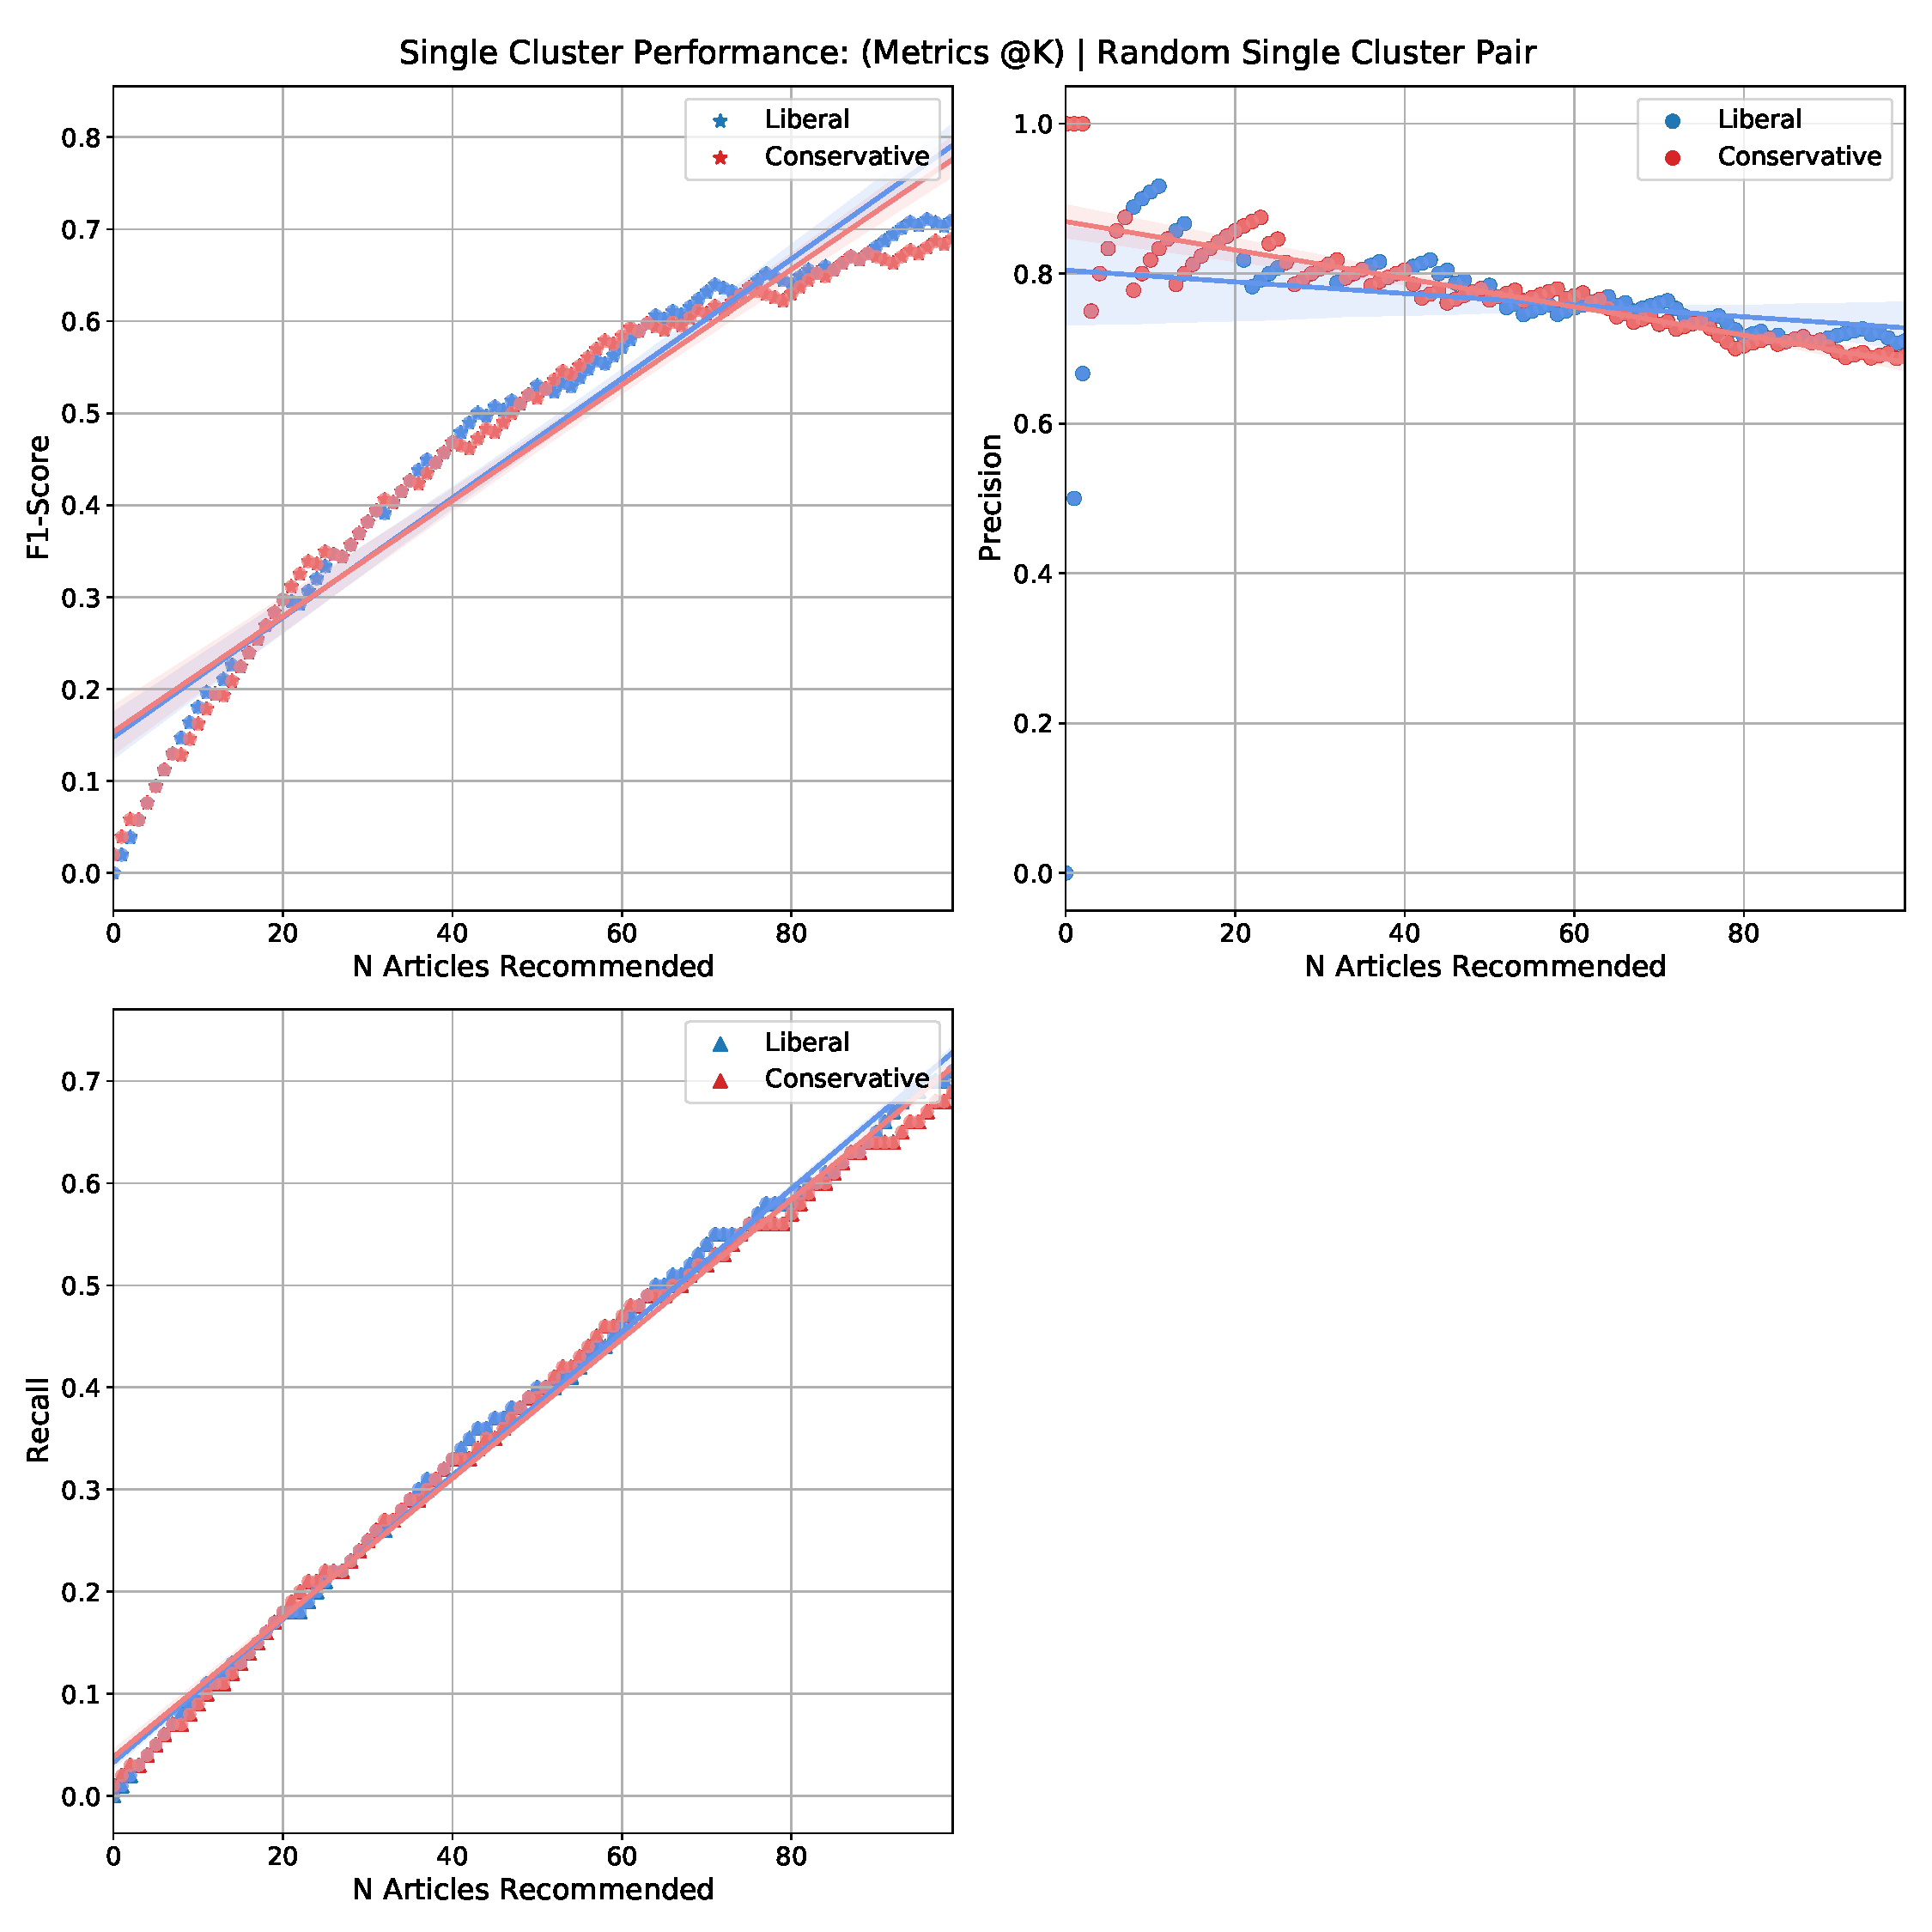
\includegraphics[width=0.6\textwidth]{Graphs/user_interaction_vs_model_performance_single_cluster.pdf}
\end{figure}
\begin{flushleft}
From the above graphs we see that \textbf{Precision@K} decreases slightly as interactions increase while \textbf{Recall@K} increases as interactions increase, the model can be optimized by varying classifier threshold, if precision is considered more important compared to recall. When we compare these scores to graphs in Baseline 2 we definitely see that the recommendation system tends to have an easier time when only one topic is concerned compared to 2 different topics, so the model is having a hard time in identifying a change in topic.
\end{flushleft}



\vspace{-1ex}
\section{Baseline 4: Varying Regularization Strength to remove Spurious Correlations}
\begin{flushleft}
We want to measure the effect of the size of regularization constant against model performance to see if removing spurious correlations helps aid model performance.

\subsection{Homogeneous Users}
\begin{flushleft}
For Homogeneous Users we see that a higher regularization constant tends to hurt model performance.
\end{flushleft}
\end{flushleft}
\begin{figure}[H]
 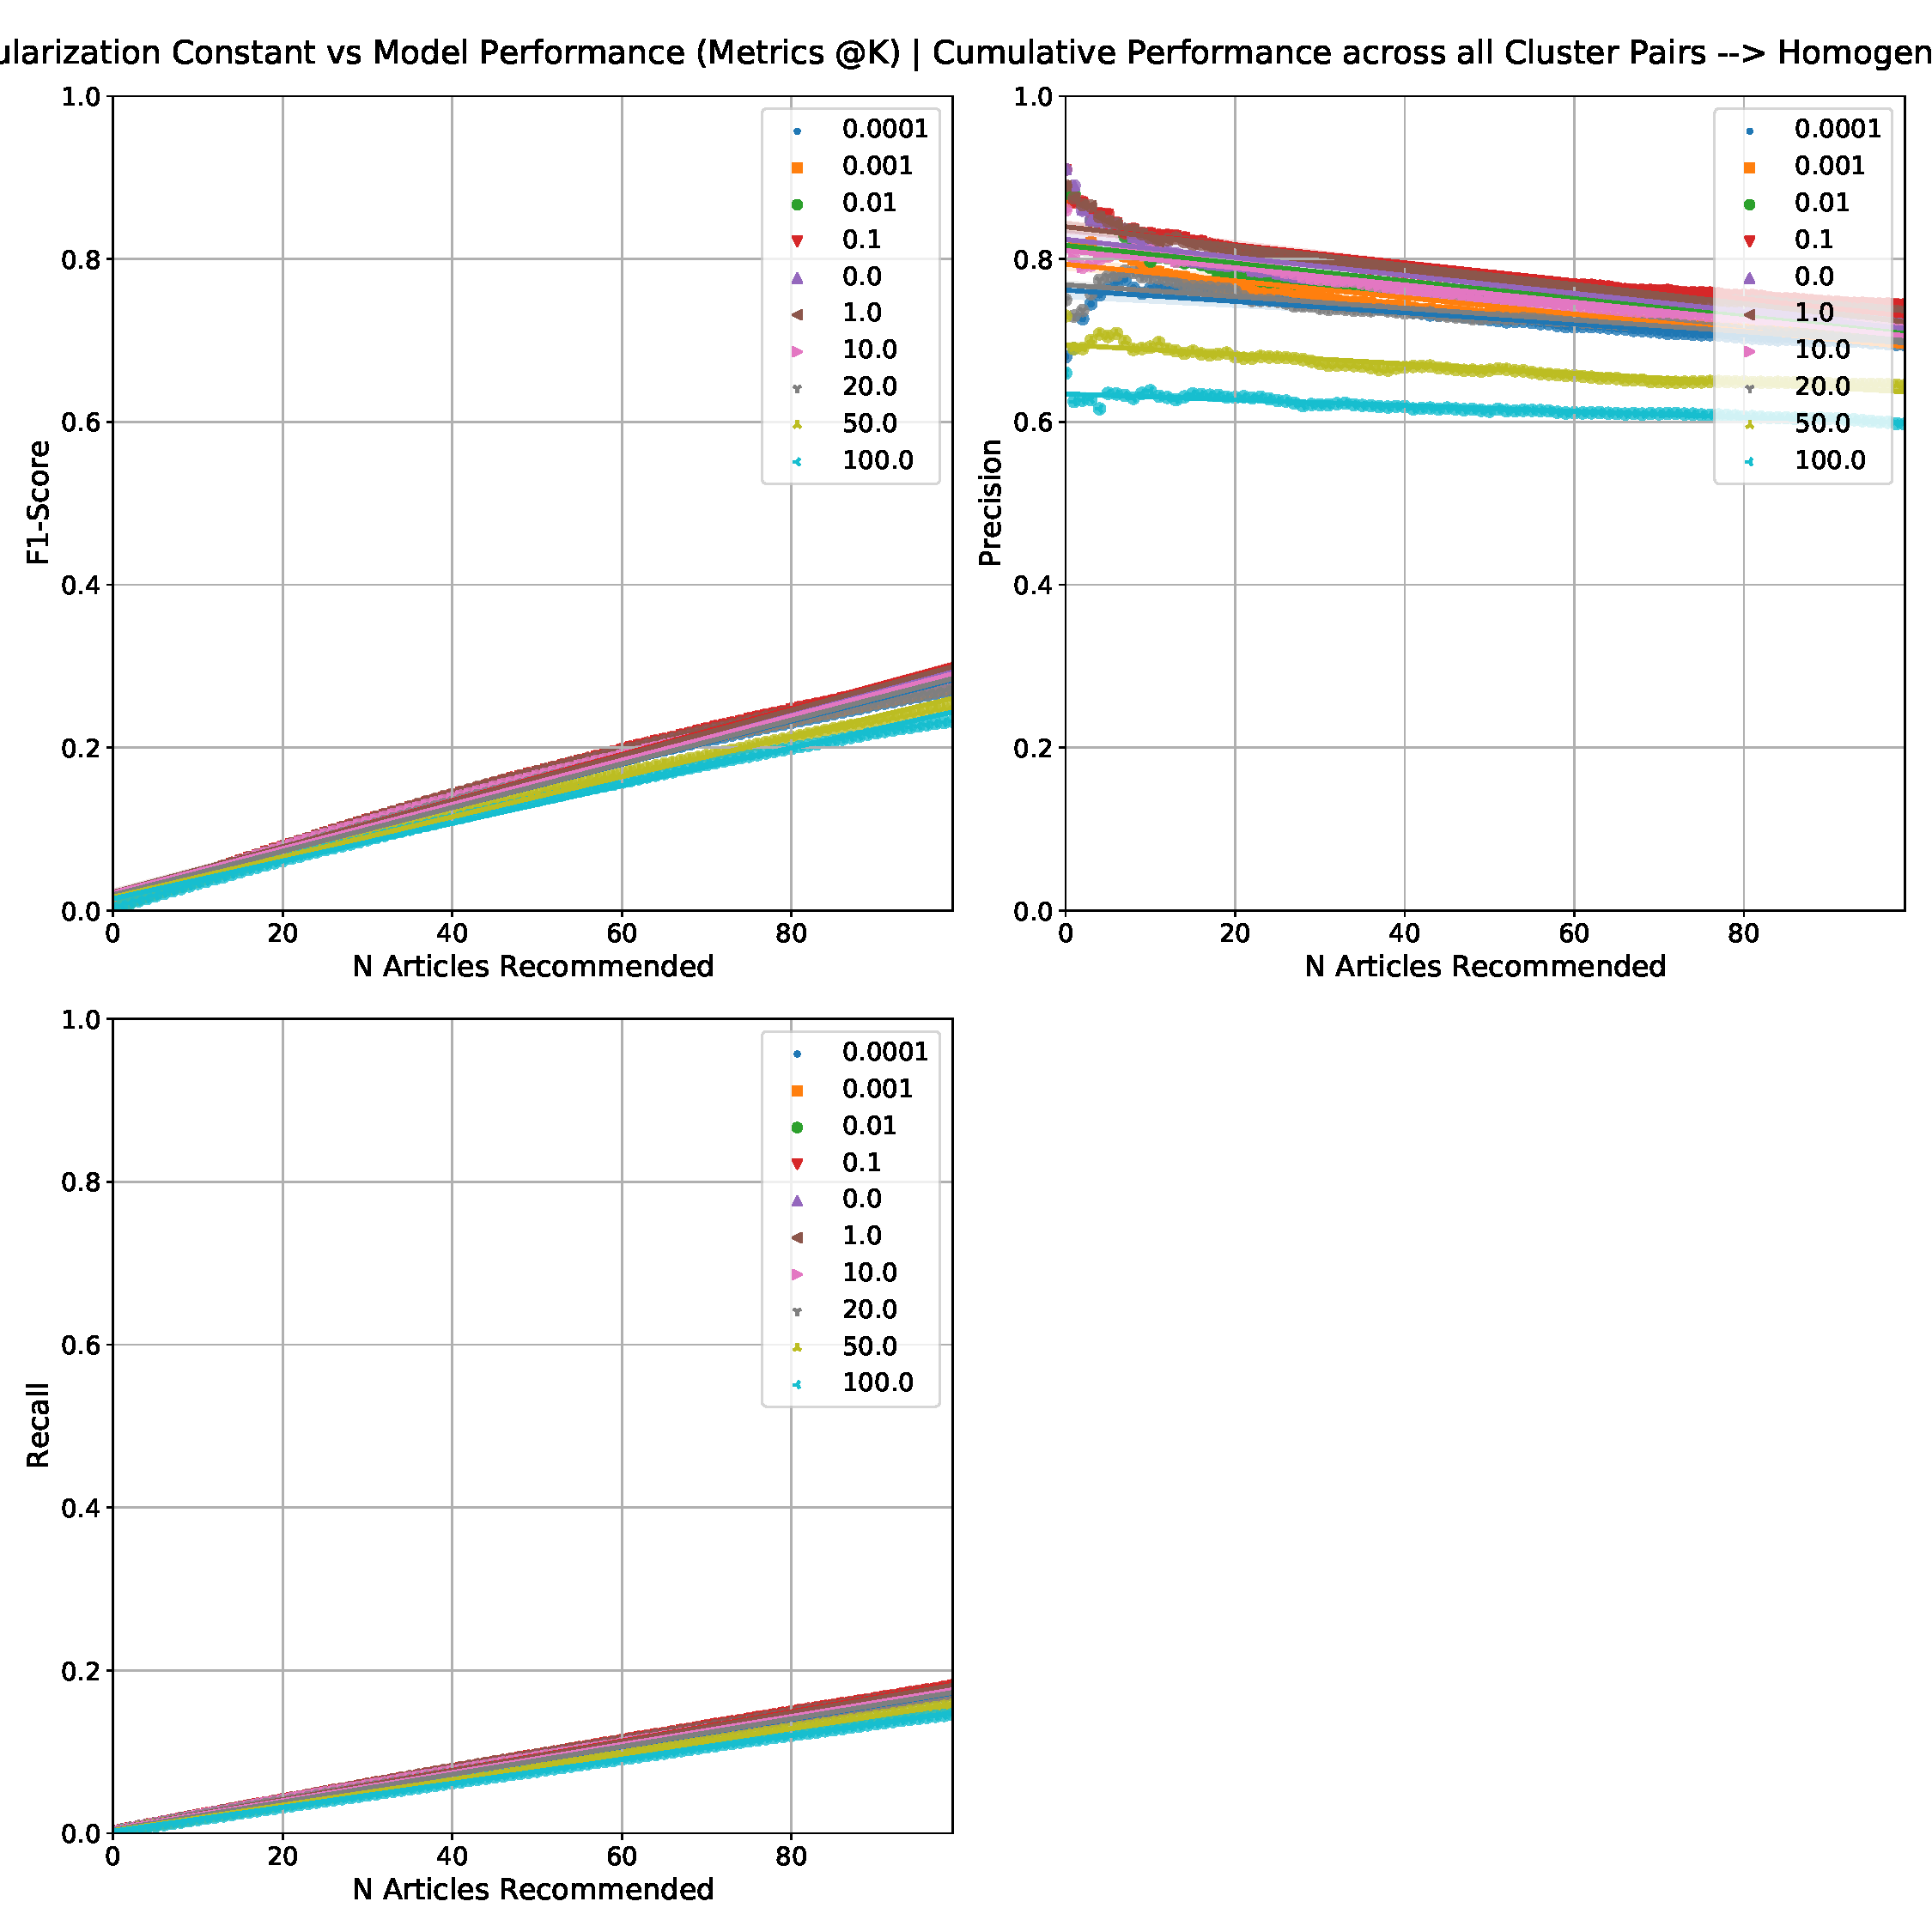
\includegraphics[width=0.6\textwidth]{Graphs/regularization_vs_model_performance_cumu_Homogeneous.pdf}
\end{figure}
\subsection{Heterogeneous Users}
\begin{flushleft}
For Heterogeneous Users on the other hand, the greater the regularization constant the better the model performs (as it can be seen across all 3 metrics), so limiting spurious correlations definitely does help in this scenario as words that overlap across stances are demoted in importance. 
\end{flushleft}
\begin{figure}[H]
 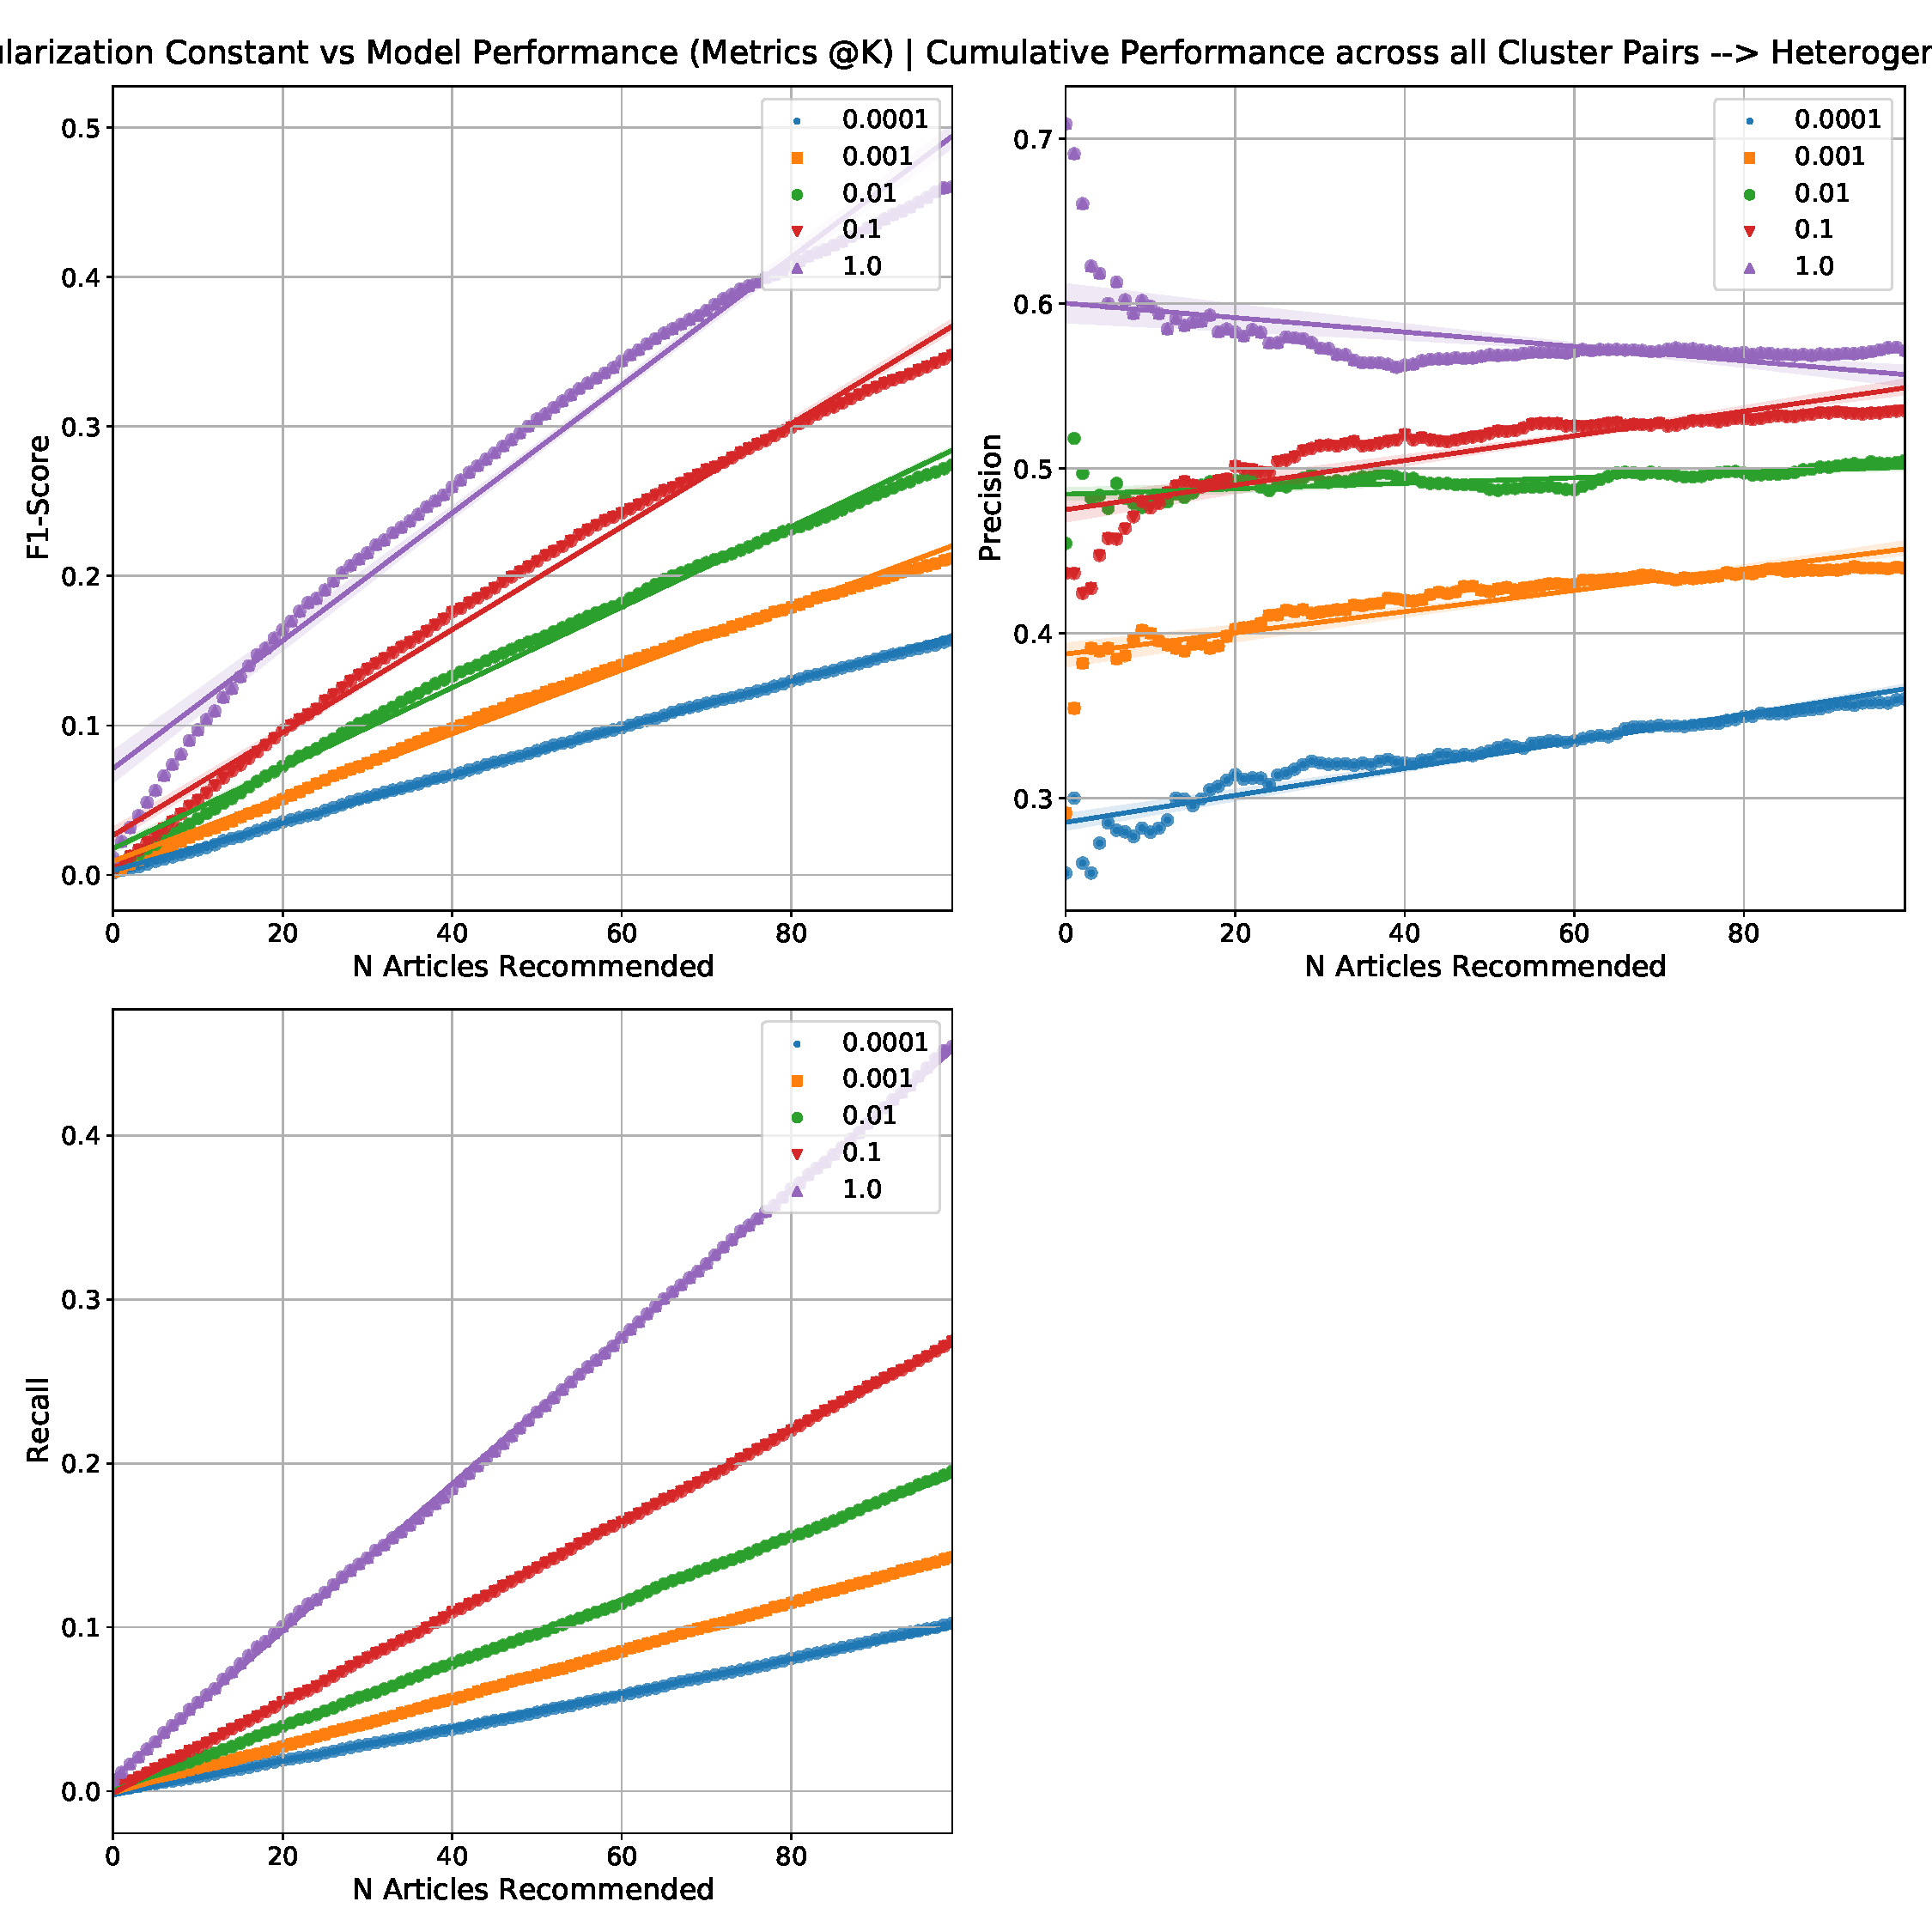
\includegraphics[width=0.6\textwidth]{Graphs/regularization_vs_model_performance_cumu_Heterogeneous.pdf}
\end{figure}



\vspace{1ex}
\section{Baseline 5: Learning Rate vs Model Performance}

\vspace{1ex}
\section{Baseline 6: Model Performance on mixed Set (Cluster 1 + Cluster 2)}
\begin{flushleft}
We want to measure how well the model would perform when an article from an unseen topic arrives along with articles from the original topic the classifier was trained on
\end{flushleft}

\vspace{1ex}
\section{Baseline 7: Utilizing Embedding Representations}
\begin{flushleft}
\begin{itemize}
    \item Context Independent Embeddings
    \begin{itemize}
         \item W2V : Word-2-vec Embeddings
        \item Glove Embeddings
        \item Fasttext Embeddings 
    \end{itemize}
    \item Context Dependant Embeddings
    \begin{itemize}
        \item BERT
        \item Elmo
        \item GPT (if available)
    \end{itemize}
\end{itemize}
\end{flushleft}



\end{document}